\documentclass[12pt, en, eng, oneside]{mgr}

\usepackage{graphicx}
\usepackage{float}
 
\begin{document}
\engtitle{
	An application for tracking the flow of resources for Bitcoin cryptocurrency \\
}
\title{Program do śledzenia przepływu środków w sieci Bitcoin}
\date{2018}
\author{Marcin Pieczka}
\supervisor{Dr inż., Radosław Michalski, Katedra Inteligencji Obliczeniowej}
\field{Informatyka (INF)}
\maketitle

\tableofcontents

\pagebreak 

\section{Streszczenie}
tekest tekst tekest tekst tekest tekst tekest tekst tekest tekst tekest tekst tekest tekst tekest tekst tekest tekst tekest tekst tekest tekst tekest tekst tekest tekst tekest tekst tekest tekst tekest tekst tekest tekst tekest tekst tekest tekst tekest tekst tekest tekst tekest tekst tekest tekst tekest tekst tekest tekst tekest tekst tekest tekst tekest tekst tekest tekst tekest tekst tekest tekst tekest tekst tekest tekst tekest tekst tekest tekst tekest tekst tekest tekst tekest tekst tekest tekst tekest tekst tekest tekst tekest tekst tekest tekst tekest tekst tekest tekst tekest tekst tekest tekst tekest tekst tekest tekst tekest tekst tekest tekst tekest tekst tekest tekst tekest tekst tekest tekst tekest tekst tekest tekst tekest tekst tekest tekst tekest tekst tekest tekst tekest tekst tekest tekst tekest tekst tekest tekst tekest tekst tekest tekst tekest tekst tekest tekst tekest tekst tekest tekst tekest tekst tekest tekst tekest tekst tekest tekst tekest tekst tekest tekst tekest tekst tekest tekst tekest tekst tekest tekst tekest tekst tekest tekst tekest tekst tekest tekst tekest tekst tekest tekst tekest tekst tekest tekst tekest tekst tekest tekst tekest tekst tekest tekst tekest tekst tekest tekst tekest tekst tekest tekst tekest tekst tekest tekst tekest tekst tekest tekst tekest tekst tekest tekst tekest tekst tekest tekst tekest tekst tekest tekst tekest tekst tekest tekst tekest tekst tekest tekst tekest tekst tekest tekst tekest tekst 

\section{Abstract}

tekest tekst tekest tekst tekest tekst tekest tekst tekest tekst tekest tekst tekest tekst tekest tekst tekest tekst tekest tekst tekest tekst tekest tekst tekest tekst tekest tekst tekest tekst tekest tekst tekest tekst tekest tekst tekest tekst tekest tekst tekest tekst tekest tekst tekest tekst tekest tekst tekest tekst tekest tekst tekest tekst tekest tekst tekest tekst tekest tekst tekest tekst tekest tekst tekest tekst tekest tekst tekest tekst tekest tekst tekest tekst tekest tekst tekest tekst tekest tekst tekest tekst tekest tekst tekest tekst tekest tekst tekest tekst tekest tekst tekest tekst tekest tekst tekest tekst tekest tekst tekest tekst tekest tekst tekest tekst tekest tekst tekest tekst tekest tekst tekest tekst tekest tekst tekest tekst tekest tekst tekest tekst tekest tekst tekest tekst tekest tekst tekest tekst tekest tekst tekest tekst tekest tekst tekest tekst tekest tekst tekest tekst tekest tekst tekest tekst tekest tekst tekest tekst tekest tekst tekest tekst tekest tekst tekest tekst tekest tekst tekest tekst tekest tekst tekest tekst tekest tekst tekest tekst tekest tekst tekest tekst tekest tekst tekest tekst tekest tekst tekest tekst tekest tekst tekest tekst tekest tekst tekest tekst tekest tekst tekest tekst tekest tekst tekest tekst tekest tekst tekest tekst tekest tekst tekest tekst tekest tekst tekest tekst tekest tekst tekest tekst tekest tekst tekest tekst tekest tekst tekest tekst tekest tekst tekest tekst tekest tekst 

\chapter{Goals}

Every process of data analysis starts with accessing the data. When analyzing Bitcoin blockchain, the first step might be the hardest one. Currently Bitcoin blockchain contains over 160GB of raw binary data, and everyone who attempts to analyze it needs to have an efficient and reliable way of obtaining it. Moreover, users should have obvious place for creating additional APIs that will be placed on the same server as the data. The reason for that is that operations requiring big amounts of data, but returning results of significantly smaller size, can be implemented more efficiently this way.
\\
\\
The goal of this work is to create an application that fulfills the following requirements: 
\begin{itemize}

\item
allows fast access to blockchain data
\item
allows access over the network
\item
updates its data in constant manner
\item
provides API for Python and R
\item
is easy to install

\end{itemize}

\chapter{Cryptocurrencies}

\section{Overview}
This chapter will explain concept of cryptocurrencies, in some cases based on example of Bitcoin. The connection between cryptography and cryptocurrencies will be shown, as well as means that are used to ensure correctness and safety of transactions.

\section{Definition}
Cryptocurrency is a digital currency in which encryption techniques are used to regulate the generation of units of currency and verify the transfer of funds, operating independently of a central bank. \cite{crypto-def}

\section{Security}
Every currency operates within its defined set of rules, and has to have means to ensure that these rules are obeyed. For regular money, as we know it today, security is provided by central authorities in multiple ways:
\begin{itemize}
\item
banknotes that are hard to counterfeit
\item
law that penalizes creating counterfeits
\item
banking systems for digital money transfer, that ensure specified rules and are secure from malicious actors
\end{itemize}

Cryptocurrencies have their own ways of ensuring their rules, but instead of central authority, those rules are ensured by cryptography and probability in a distributed system.

\section{Cryptography}
Cryptocurrencies are in big part based on cryptography to ensure the rules at which they operate. Cryptography helps not only to ensure that fraudulent and malicious operations can't have their place, but as well to establish rules of creating new units of those currencies. 

Cryptography is a field of knowledge that has its focus on protecting information from unauthorized access as well as providing means to authenticate and ensure integrity of message.

Cryptography can be classified as:

\begin{itemize}
\item
Symmetrical - Information is encrypted and decrypted with the same key, with this type of encryption arises problem of transferring the key.
\item
Asymmetrical - Information is encrypted with different key than the key that is used for decryption. One key is usually called the public key, and is used to encrypt messages. Because public key cannot be used to decrypt message it can be shared freely without concern. Second key is called private key an is used to decrypt messages. Private key should never be shared, everyone possessing that key can decrypt messages encrypted with related public key.
\end{itemize} 

Public key cryptography was developed in 1970s and is widely used to ensure security of information today. Mathematical functions were discovered that are easy to calculate in one way, but nearly impossible to calculate in reverse. Bitcoin uses elliptic-curve functions as a base of calculating public key.\cite{bartek}

Aside of encryption, Bitcoin uses cryptographic hash functions in its inner workings. Cryptographic hash functions map strings of arbitrary length to constant number of bits called digest, typically from 128 to 512. 

One of the main properties of hash functions is that they work one-way only. This means that for given hash digest it is impossible to find original message, but creating hash is easy. Another important property of hash functions is that for different messages, output should be different. This property does not hold in theory. Because output space of hash function is finite, and input space being virtually infinite, there must exist such messages that while being different, their hashes are identical. In practice output space is so large that finding so called collisions is nearly impossible. Therefore when hash digest is identical for two messages, those messages are assumed to be identical as well.  \cite{hash-functions}


\chapter{Bitcoin}

\section{Overview}

This chapter explains Bitcoin protocol, communication between nodes, transactions and creation of blocks.

\section{Network}
Bitcoin is distributed network and there are no authoritative nodes. The exception are servers that are used by new Bitcoin nodes to discover other nodes, but they will not be discussed. Reason for it is that essentially they are not part of Bitcoin network, and if those servers fail, nodes will use other methods for discovery. 

There are two types of information that nodes share between them: transactions and blocks. \cite{bitcoin-paper-1} Those entities will be discussed in separate sections.

\section{Transactions}
Transactions in Bitcoin are used to transfer value between owners. Single transaction describes inputs from which resources are being transfered, and outputs to which those resources are being transfered. All the resources from the inputs are being transfered to the outputs, unused resources are transfered to the miner which is known as transaction fee.

Inputs are described by reference to output of previous transaction. To reference output of transaction, hash of transaction is needed as well as index of output, numbering of outputs starts with 0. Additionally for each input, there is attribute that makes it possible to verify that resources are transferred by their rightful owner. \cite{bitcoin-transaction}

Outputs of transaction specify number of BTC that is being transfered to that output, and a script that defines way of accessing those resources. 

As have been stated outputs define way of accessing resources, and inputs provide values that unlock those resources. This is done with scripting system.

\section{Scripts}
In Bitcoin providing access verification is done with scripting system. Scripts in Bitcoin are programs, written in non Turing complete language, that when processed determine whether access to resources protected by script is granted or not. \cite{bitcoin-script}

Because this system is very versatile, granting access to resources can require e.g. providing multiple keys, providing password, can be granted to everyone etc. 

Although script system allows for many methods of authentication, one of them is used in most of the transactions. In this method is often called "pay-to-pubkey-hash". Script field of transaction output specifies hash of public key and requires anyone wishing to spend this output to provide signature and public key. Hash of public key must be equal to hash provided in output. Signature, which proves that spender owns the private key, must be correct.


\section{Blockchain}
Blockchain in Bitcoin is data structure that holds every transaction that had taken place since beginning of Bitcoin network. It consists of blocks of transactions, with each block holding in itself hash of previous block. Every Bitcoin node, after it has synchronized with the network, holds entire blockchain in its memory.

One notable property of this data structure is that modification of single block would require modification of every block that followed. This property of blockchain comes from the fact that modification of block, changes its hash, and as mentioned before blocks contain hash of previous block. This of course would require modification of previous block hash field in following block. 

Because of restrictions imposed on block creation, creating blocks is highly time consuming, thus modification of block that had been followed by 6 other blocks is considered impossible without consent of large portion of miners.

\section{Mining - block creation}
Mining in Bitcoin is the process of block creation. One of the most interesting properties of valid block is that its hash starts with certain amount of "0". Number of "0" needed at beginning of correct block is being adjusted every 2016 blocks, so that rate at which blocks are being mined is approximately 1 block per 10 minutes. To achieve needed hash, attribute named "nonce" is set in trial and error manner. Everyone who wishes to create new block will need to:

\begin{itemize}
\item
listen on the network for new transactions
\item
gather transactions into block
\item
set all attributes of block like previous block hash, transaction count etc.
\item
set value of "nonce" attribute
\item
calculate hash of block
\item
if hash starts with needed number of "0" than propagate block through the network, otherwise set "nonce" to different value and continue process till finding correct value or till some other miner finished 
\end{itemize}

Naturally, process described above is simplified. There are some nuances, e.g. "nonce" attribute is 32 bit integer, and nowadays more often than not there is no such value of that attribute that results in correct hash. Miners in such situation apply other techniques to find correct hash. Nonetheless this is level of detail this work does not operate on.
 
Incentives for mining blocks are transaction fees and block rewards. Transaction fee is any unspent output in a transaction. For instance when 0.9 BTC is sent from output that holds 1 BTC, unspent output equals 0.1 BTC. This unspend output can be transfered to address controlled by miner.  
Another incentive, block reward, is last transaction in the block which creates new coins and transfers them to address specified by miner. Amount of BTC in block reward started at 50 BTC, and halfs every 210000 blocks \cite{currency-supply}


\chapter{Alternative software providing similar features}

\section{Overview}
This chapter describes software that is similar to what will be designed and implemented in this paper. These descriptions go through features, advantages and disadvantages of those applications. 

\section{blockchain.info}

Web application blockchain.info provides free access to Bitcoin blockchain data by either website, JSON API or APIs dedicated to specific languages including Python. Blockchain.info does not have dedicated support for R. Number of requests is limited.
\\
\\
Relevant APIs provided by blockchain.info:
\begin{itemize}
\item
getting single block, by block hash
\item
getting single block, by hight
\item
getting multiple block headers
\item
getting single transaction, by transaction hash
\item
getting all transactions of single or multiple addresses


\end{itemize}

Most common usage scenario in analytic context is getting range of blocks, for example all blocks from 10.04.2017 to 20.04.2017. Nonetheless, blockchain.info does not provide simple way of getting such data. To achieve this, thousands of requests to API providing us with single block data is needed, and this is not fast enough.

Another and the biggest problem is the API call limit that would make working with this application impossible for larger queries.

\section{blockexplorer.com}

This web application is very similar to blockchain.info in almost every aspect, although there are some differences. Data is accessible either by website or by JSON API, but there is no Python or R API provided. Set of APIs is almost identical to blockchain.info and does not provide easy way to get multiple blocks. The main difference is that there is no official API call limit, but because it is external tool, it means that such limit can appear every moment.

\section{libBitcoin-database}

\begin{verbatim}
https://github.com/libbitcoin/libbitcoin-database Last visited 25.04
\end{verbatim}

This piece of software, after installation builds in-memory database of Bitcoin blockchain, its description promises high performance. Because of almost non existing documentation, it is hard to describe its features in depth.
\\
\\
Although this software is actively developed, and at first sight it might seam like solution that fits needs of users, some problems can be found. One drawback is coming from its biggest selling point - being in-memory database makes it requiring large amounts of RAM. This problem makes it not viable for hardware that is accessible for the average user. Next problem lies in its API that allows connecting to the database only via C/C++ library, which would make usage in R and Python at least problematic. Another problem is already mentioned lack of useful documentation, which would make the usage largely troublesome.

\section{BitcoinDatabaseGenerator}

\begin{verbatim}
https://github.com/ladimolnar/BitcoinDatabaseGenerator Last visited 25.04
\end{verbatim}

BitcoinDatabaseGenerator is a data transfer tool that can feed SQL database with blockchain data. It was written in C\# and as its author states, it is only meant to be run on Windows machines. From the documentation we know that this software should be ran every time we want to update our database. Database schema that is created after update operation, consists of separate tables for blocks, transactions, transaction inputs and so forth. Such database schema would require joining tables in multitude of usage scenarios, which is known to be slow operation.
\\
\\
Although connecting to SQL database from both R and Python is easily achievable, working with SQL databases in such case might be cumbersome. Abstracting away relational structure of data to objects might be needed when working with SQL database. 


\chapter{Design}

\section{Overview}
This chapter goes through design process in detail. Design starts with describing users and their needs. Than system is described as black box, with its inputs and outputs. After that design flows as questions and issues arise. 

\section{User requirements}

\subsection{Users description}

Requester of this software is Ph.D. working at university. He is interested in networks that emerge between cryptocurrencies users. The cryptocurrency that he researches the most is Bitcoin, because of its wide adoption which leads to his research having bigger impact. He believes that science is group activity, and thus he wants knowledge to be shared in efficient way. He has created group of people working on this subject at his university, and actively pursues better communication and collaboration with similar groups at other universities. Problem he and his peers faces is lack of standard way to share common analytic solutions, which hinders accumulation of knowledge. With such place, as he believes, common analytic tasks would not have to be implemented over and over by separate researchers. One of common tasks that he notices to be implemented over and over is acquiring Bitcoin data.  

\subsection{User stories}

The following sentences sum up the discussions with people that consider using this system.

\begin{itemize}
\item
As a user, I want to access blockchain data from my Python/R script so that data analysis and data accessing can be made in the same code.
\item
As a user, I want the data be in a format idiomatic to Python/R so that I don't have to convert it myself.
\item
As a user, I want easy access to block data by specifying range of time or block height so that I can spend my time working with the data, and not with accessing it.
\item
As a user, I want the installation not to require complicated operations so that I can do it without specialized knowledge.
\item
As a user, I want to be able to run this software on my linux server so that I don't have to learn new operating system to be able to use it.
\item
As a user, I want fast access to the data so that my analytic scripts will be pleasurable to work with.
\item
As a user, I want to have obvious place to create my own APIs on server so that my new data hungry features can be placed on the same server as data for better performance.
\end{itemize}



\section{System inputs and outputs}

In this section inputs and outputs of the system will be specified. This will then help to discover what transformation the input data will undergo, and what components are needed to provide outputs efficiently. Here will be considered only part of the project that is responsible for serving data, not the part that will be responsible for hosting future APIs.

\subsection{Inputs}
\subsubsection{Bitcoind BLK files}
The only source of Bitcoin block data will be BLK files, stored by full Bitcoin node. Daemon process bitcoind gets blocks from neighboring nodes, and stores them in data directory. The BLK files in default configuration store up to 128MB of raw network format block data. Blocks are stored in order in which they come from network. Library's that handle parsing BLK files exist, so accessing this data should not be a problem.

\subsubsection{Request for blocks} This request will be the way user communicates with the system. In this request user will specify which blocks he wants to receive. Usually those will be blocks from specified range of time, or range of height.

\subsection{Outputs}
\subsubsection{Response on request for blocks} This response will contain block data in format either native to Python/R or JSON.


\section{Persistence}
The fact that transaction sender address is not stored in Bitcoin blocks directly, but by reference to other transaction, creates responsibility for the system. This responsibility is to discover addresses by finding referred transaction, and getting the address of recipient. This of course requires substantial amount of time which should not be added to the time of user waiting for his response. 
\\
Additional thing to consider is the time needed to transform raw binary Bitcoin block to widely used data format such as JSON. Knowing this we will get to the conclusion that we need some type of persistence. Although some custom way to store this data might be better suited for our needs, database will be used, because of constraint of time available to build this solution.

\subsection{Database operations}
Let's consider database operations that will need to be fast, and those that are not so important in this regard.
\\
\\
Least important operation will be data addition. End user will not be performing these operations, and its performance will be of least priority.
\\
\\
Most important operation will be querying blocks, by theirs hash, time, and other attributes, especially querying for range of consecutive blocks described by time frame or height range.
\\
\\
Another important operation is getting transactions by hash. This operation will be needed for discovering addresses of transaction senders. Although this operation will not be in usage scenarios started by end user, the number of such operations needed to discover sender address of every Bitcoin transaction makes it crucial for this it to be fast.

\subsection{Database choice}
At the beginning let's simplify the choice between RDBMS (Relational Database Management System) and NoSQL databases. Out of many NoSQL possibilities, MongoDB (web page: www.mongodb.com) have been chosen, based on initial research of different NoSQL systems strengths and weaknesses.


Let's lay out some facts that will help to decide whether to use relational database, or MongoDB.

\begin{itemize}
\item 
Storing blocks in RDBMS in multiple tables, for instance table for blocks and table for transactions, would require joining those tables which could be slow operation.
\item 
To achieve fast querying, the data should be strongly denormalized.
\item
Storing blocks in RDBMS in one table can be impossible in many systems, due to attribute count limit.
\item 
Comparable performance can be achieved with MongoDB and RDBMS, but MongoDB makes storing denormalized data idiomatic.
\item
MongoDB have APIs for Python and R that makes data available as objects.
\end{itemize}

Based on these facts, the database that will be used is MongoDB. This choice will provide easy access to the data from Python and R code, and achieving needed performance will come without problems.


\subsection{Database structure}
 
Collections in MongoDB don't have structure defined upfront. To have mandatory attributes, actor responsible for data insertion needs to enforce it. Because of this, writing about database structure is not most accurate term. It is easier to think about it as structure of data, and in my system the structure of data will not change in big degree compared to form it will be obtained from blocks. The only difference is, that by default, Bitcoin transactions don't specify address of sender. Additionally attribute have been added, that is the time that had passed between receiving resources which were input of transaction, and that transaction.

One document in MongoDB collection will be one Bitcoin block, its attributes are:
\begin{itemize}
\item
bits - current target in compact format \cite{bitcoin-wiki-bha}
\item
difficulty
\item
hash - hash of this block
\item
height - number of blocks before this block in blockchain
\item
merkle root - hash based on all transactions of block
\item
n tx - number of transactions
\item
nonce - value set by miner to achieve needed block hash
\item
prev hash - hash of previous block
\item
size
\item
timestamp - time at which block had been mined
\item
transactions - list of transactions with each transaction consisting of:
\begin{itemize}
\item
hash - transaction hash
\item
inputs - list of data regarding addresses from which resources had been transfered, consisting of:
\begin{itemize}
\item
transaction hash - hash of transaction in which sender of this transaction got resources spent in this transaction
\item
transaction index - points to certain output in transaction described by previous attribute
\item
output timestamp - additional value described before this list of attributes
\item addresses - list of addresses, each containing:
\begin{itemize}
\item
address
\item
hash
\item
public key
\item
type
\end{itemize}
\end{itemize}	
\item
outputs - list of data regarding addresses to which resources had been transfered, consisting of:	
\begin{itemize}
\item
value
\item addresses - list of addresses, each containing just like in inputs:
\begin{itemize}
\item
address
\item
hash
\item
public key
\item
type
\end{itemize}
\end{itemize} 	
\end{itemize}
\end{itemize}

 

\subsection{Database indexes}

Database indexes serve purpose of making queries faster and more efficient on cost of space and data insertion time.
Because performance of queries is one of key user needs, and space and data insertion time are very low on priority list, the indexes will be added to all of the fields that data will be queried by.

Indexed attributes:
\begin{itemize}
\item
block hash
block timestamp
transaction hash - needed internally for discovering input addresses
\end{itemize} 


\section{High level architecture}
This system will consist of separate entities, that will have their own, well defined responsibilities. This will make those components and overall system easy to understand and maintain.
\\
\\
System will consist of:
\begin{itemize}
\item
Bitcoin node with its data directory
\item
database for storing processed blocks
\item
process constantly updating database with new blocks that are gathered by Bitcoin node, which will be referred to as database updater
\item
web application ready to implement complex functionalities in
\end{itemize}

\begin{figure}[H]
  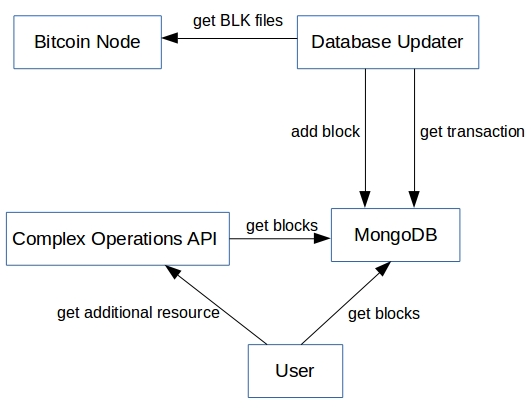
\includegraphics[width=0.8\linewidth]{component-diagram.png}
  \caption{System components and their communication}
  \label{fig:system-components-and-their-communication}
\end{figure}

\subsection{Database Updater}
This component will be responsible for:

\begin{itemize}
\item
parsing raw Bitcoin blocks collected from BLK files
\item
discovering transaction sender address by transaction output referred in its input
\item
adding blocks to database
\item
administering the database, namely adding indexes in the best moment
\end{itemize}

Although this components performance does not influence user wait time, it influences time needed to get to the point at which most of the recent blocks are in the database. Because of large amount of data that needs to be processed and inserted to database, optimizations are necessary to finish initial data load in reasonable time.

The main bottleneck is discovering sender address. Nowadays, one block holds about 2000 transactions, so to process one block with simplest algorithm, database updater would have to ask the database about 2000 times for transaction for every processed block. This would lead to very poor performance. Because it would require to much memory for database updater to remember every transaction it have processed, it will remember some constant number of last processed transactions.

\subsection{Complex Operations API}
Reason for this component to be requested is the fact that when there is a group of people researching common field, there is big overlap in needed functionalities. When researcher gets to the point where he needs functionality that he doesn't have, he will implement it himself. The problem is that very often the same functionality was implemented by one of his peers, and this component is meant to solve this problem. 

In order to incentivise users to use this API, in regard of developing new functionalities, it needs to be at similar level of complexity as developing those functionalities locally, and it is crucial to consider it during design.

Complex Operations API will be web service, which in response to its users request will return JSON data. At the main page will be located descriptions of implemented functionalities with URL's needed to access them. There will be one functionality implemented in this service which purpose will be to handle to the users a well working example of something similar to what they will be implementing.   

\section{Deployment}

The main property of software, that can be accomplished with well chosen deployment and packaging, are simplicity of use and cross-platform possibilities. Those can positively influence adoption rate of this solution in perspective of both usage and further open source development.

For this project docker containers will be used (web page: www.docker.com), which will help in keeping components decoupled, and will make installation process easy to follow. 

Installation process should consist only of installing full Bitcoin node, docker, running one custom script and setting up simple configuration (database credentials, etc.).

All the containers will be connected to the same private network, so that communications between them will lack any complexity.

\chapter{Implementation}

\section{Overview}
This chapter shows most notable implementation details, selected by their importance to the system. Implementation starts with deployment which usually is the last concern, but in this case it has guided whole implementation process. Later, implementation of system components is described.

\section{Install.sh}
This tour of implementation starts with the installation script, because knowing its content will provide knowledge of containers set up, data flow between containers, an overview of whole system.

Install.sh starts with reading configuration from file "config.conf" in which following things are being set up:

\begin{itemize}
\item
database credentials for administrator and user with read-only privileges
\item
port at which the database will be reachable
\item
data directory of Bitcoin node
\item
directory at which database data will be stored
\item
transaction cache size
\end{itemize} 

After configuration is loaded, network is being created, and building and starting of containers begins.

\subsection{Database container setup}
For database container configuration will be shown, so that readers without experience with docker will have chance to see how such configuration looks.

\begin{verbatim}
docker run -d \
    --name btc-blockchain-db \
    -e AUTH=yes \
    -e MONGODB_ADMIN_USER=$db_root_username \
    -e MONGODB_ADMIN_PASS=$db_root_password \
    -e MONGODB_APPLICATION_DATABASE=bitcoin \
    -p 0.0.0.0:$db_port:27017 \
    -v $database_dir:/data/db \
    --network=btcnet \
    aashreys/mongo-auth:latest
\end{verbatim}

Database container is build on "aashreys/mongo-auth:latest" docker image, which lets us create MongoDB database with enabled authentication (by default in MongoDB authentication is not enabled).
Admin user credentials are being set, but credentials of user with read-only privilege can't be set here, because before-mentioned image does not support such action.

There are couple other things in this configuration worth noting, namely "-v" flag creates volume for container and its purpose comes from the fact that docker containers should be possible to be killed without any loss. With volume set up, when we kill our database container and run it again, the database data will persist.

Another important thing is setting up common network for all the containers, here it is accomplished with flag "--network". With network configured, DNS is set up automatically and it is possible to refer other containers by their names. For instance running 
\begin{verbatim}
ping btc-blockchain-db
\end{verbatim}  
from within other container connected to the same network will send messages correctly

\subsection{Database updater container setup}
Before database updater docker image can be ran, it needs to be created first. To create docker image, configuration needs to be written in file named "Dockerfile", than command "docker build" is used to build image. With image ready it can be ran in the same way previously described image was.

Dockerfile for database updater:
\begin{verbatim}
FROM python:3

COPY requirements.txt ./
COPY ./src/ /src/
RUN pip install --no-cache-dir -r requirements.txt

# forked version from 22.03.2018
RUN pip install https://github.com/MarcinPieczka/python-bitcoin-blockchain-parser/archive/master.zip

RUN mkdir /btc-blocks-data/

EXPOSE 27017

CMD [ "python", "-u", "/src/update_database.py" ]
\end{verbatim}

Dockerfile starts with base image that is being used, here it is "python:3" image that contains as its name suggests python3 installed.
Next two lines copy needed files to the container, than libraries are installed, containers port is exposed for communication with database, and in the last line my application is being started.
\\
\\
Using docker makes it easy to create installation process repeatable and independent from environment, so that running software will have the same effect on every machine it is being ran (to some extend naturally). 

\subsection{Complex Operation API container setup}
This container is based on "tiangolo/uwsgi-nginx-flask:python3.6" which have all the basic elements needed to run flask application already configured. The only non standard configuration that needed to be done is setting timeout in Nginx web server to larger value. By default timeout is 60 seconds, but because of type of operations that this application is made for, this is not enough.  

\section{Database updater}
This container as stated before is responsible for database, and in more detail it is responsible for both putting data to it and for managing its configuration. In regards of managing configuration of database, this module takes responsibility for everything that could not be achieved in docker command, and that is:

\begin{itemize}
\item
Creating user with privilege to read the database, but not to modify it. This account will be used by end user.
\item
Creating database indexes for block height, block timestamp and transaction hash.
\end{itemize}

All this is being done in separate module responsible only for database - "mongo.py". Other than caring for database configuration, it abstracts away connecting and loading data to the database. This module uses library "pymongo" in version 3.6 to connect to database.
\\
\\  
Data insertion took the most effort to develop, and is the most complex part of the system.

All of Bitcoin BLK files processing is done with "blockchain-parser" library, but not the official release, but version straight from their git repository (web page: www.github.com/alecalve/python-bitcoin-blockchain-parser). The reason for this is that changes in Bitcoin are far more frequent than releases of this software, and some features of Bitcoin were not supported in official version. The version that is being used does not support BIP-0173 (BIP stands for Bitcoin improvement proposal) so discovering addresses from transactions using techniques described in it cannot be done. 
\\
\\
Processing and loading data can be broken into these steps:
\begin{itemize}
\item
Initial parsing of BLK files contained in Bitcoin data directory. Only headers of blocks are parsed, to get hash of block, and hash of previous block.
\item
Representation of blockchain is created, to get to know the order of blocks, and to know which blocks are in the main chain.
\item
One by one, starting from the block next after last inserted, blocks are fully parsed. Their transactions are cached, and input addresses are being discovered. Those addresses are being discovered first by looking into cache, than if cache does not contain needed transaction, the database is being asked.
\item
last step is inserting processed block into database.
\end{itemize}

Of course there is more complexity hidden inside those steps, like handling exceptions from blockchain-parser library. The reason there are exceptions while parsing Bitcoin blocks is that Bitcoin transactions do not have to be fully valid. Many transactions exist with errors, and although they are of no interest to the system, they need to be recognized and handled properly.

\section{Complex Operation API}
This component was implemented in Flask framework (web page: www.flask.pocoo.org), which was chosen for its simplicity. Simplicity is well needed in application that users, who very often don't have experience with web applications, will extend with their code. 

Main page is made purely in HTML and CSS, for the sake of before mentioned simplicity.

Two exemplary functionalities have been implemented, one of which, because of its lack of complexity, will be a good way to show advantages of Flask.
\begin{verbatim}
@app.route('/api/last_block')
def _last_block():
    return dumps(mongo.db.blocks.find().sort([('height', -1)])[0])
\end{verbatim}
In this code first line specifies address at which service will be available, second one is declaration of function, and the last one is its implementation. This function connects to the database with previously created "mongo" object, finds last block in the database, converts it to JSON with "dumps" function and returns.
\\
\\
The second functionality is surely more complex. First of all lets notice that we can look at Bitcoin transactions as graph. Every transaction has its input and output, the addresses of inputs and outputs are vertices of the graph, and transactions are the edges between them. My second functionality as input takes two parameters which specify block range by hight, than creates graph out of transactions found in specified blocks using iGraph library. After creating graph it separates unconnected graphs and returns array of count of vertices in each graph.

The choice of this functionality was not random. Operations on graphs are very common when analyzing Bitcoin transactions.

At the end it needs to be said that although that application by itself is easy to understand and in this regard it will be easy for users to add their code to it, the deployment with docker makes it not so easy to use as a developer. Biggest drawback of docker is relatively slow startup. When some portion of code is written into this container, and it needs to be ran for testing, process of building image will take about 15 s (time based on personal observations) 

\chapter{Functionality testing}

\section{Getting blocks by height}
Getting Bitcoin blocks by their height has been identified to be one of the most needed way to query blockchain, and its performance is of high priority.
 
\subsection{testing on the same machine as database} 

\subsubsection{consecutive blocks test}
results:
\\
blocks between height 0 - 99: \quad \quad \quad \hspace*{2em} 0.0035 s\\
blocks between height 100000 - 100099: \quad 0.0065 s\\
blocks between height 200000 - 200099: \quad 0.48 s\\
blocks between height 300000 - 300099: \quad 1.7 s\\
blocks between height 400000 - 400099: \quad 7.9 s\\

\subsubsection{spread blocks test}
results:
\\
100 blocks spread between height 0 - 100000: \quad \quad \quad 0.49 s\\
100 blocks spread between height 100000 - 200000: \quad 1.2 s\\
100 blocks spread between height 200000 - 300000: \quad 1.6 s\\
100 blocks spread between height 300000 - 400000: \quad 3.5 s\\

\subsection{testing with accessing database by network}

\subsubsection{consecutive blocks test}
results:
\\
blocks between height 0 - 99: \quad \quad \quad \hspace*{2em} 0.097 s\\
blocks between height 100000 - 100099: \quad 0.15 s\\
blocks between height 200000 - 200099: \quad 5.1 s\\
blocks between height 300000 - 300099: \quad 13 s\\
blocks between height 400000 - 400099: \quad 51 s\\

\subsubsection{spread blocks test}
results:
\\
100 blocks spread between height 0 - 100000: \quad \quad \quad 2.9 s\\
100 blocks spread between height 100000 - 200000: \quad 5.7 s\\
100 blocks spread between height 200000 - 300000: \quad 15 s\\
100 blocks spread between height 300000 - 400000: \quad 42 s\\

\subsection{Result interpretation}
When comparing results for tests ran locally and over network, about ten fold difference in time can be noticed. This means that performance of database is not a bottleneck and there is no need for further optimizations.

Another noticeable thing is that query time highly depends on height of blocks requested. The reason for this is the fact that, because of gradual adoption of Bitcoin, the average number of transactions in blocks had grown over years. 

\section{Getting blocks by timestamp}
Because querying by hight and by timestamp should not give different results, only one test will be performed.
\\
\\
result of run over network:
\\
blocks between timestamp 2016-02-25 16:24 - 2016-02-26 07:23: \quad 58 s

\subsection{Result interpretation}
Because range of time that was tested fully corresponds to getting blocks by hight with range of height being from 400000 to 400099 we can compare those results. There seams to be no significant difference in performance between getting by height and by timestamp.

\section{Complex operations API}
In functionalities prepared in this component, performance is not main goal. All available services will be requested, to see if results are satisfying.

\subsection{Getting last block}
service is located at http://base-address/api/last\_block and calling it returns JSON data:
\begin{verbatim}
{
    "_id": {
        "$oid": "5ae122209043650001213f12"
    },
    "hash": "000000000000000000c0af3be64d9a335968225b35f9fb102d4962c0ff2558c2",
    "version": 536870912,
    "height": 496509,
    "prev_hash": "000000000000000000384595a7dc898a505d5c131dffa1c55431dc73cffe2355",
    "merkle_root": "9df11de2a46b352591f5980d63929c68d9af01bc2e494f4b350ae697809773ac",
    "timestamp": {
        "$date": 1511869304000
    },
    "n_tx": 2425,
    "size": 1079456,
    "bits": 402706678,
    .
    .
    .
}
\end{verbatim}

\subsection{Getting count of maximal connected graphs by height}
service is requester with address
\\ \verb|http://base-address/api/count_separate_graphs?height_from=100000&height_to=100500|
and in this case it returns [1701,74,42,39,21,20,20,19,17,...] which means that biggest connected graph that can be made from transactions with height from 100000 to 100150 has 1701 vertices, and so forth.


\chapter{Beyond implementation}

\section{Usage}
After implementation finished, described software was used by fellow student in research he conducted for his master thesis. In his research he performed cluster analysis of Bitcoin transactions. His opinion of this software, as he stated, had fully met his needs, but he expressed his concern for security of current authentication system. In his opinion if someone unauthorized would acquire credentials, denial of service attack could be performed.

\section{Problems}
In this section, several issues this software have will be addressed.

\paragraph{Lack of support for newest blocks} is the problem with biggest impact on usability of this software. Without sorting it out some users will find this system incapable of finding their needs. 

\paragraph{Authentication by one set of credentials} can lead to security issues. At current version, every end user is provided with credentials to access functionalities. Those credentials are identical for every user, and provide read only access. One problem with that solution is that when one user uses to much resources, it is hard to find who this user is. Another problem arises when administrator of system wants to restrict access for some users. In this case he would need to create new credentials and distribute them to all users that should have access to the system.

\paragraph{Maintenance} can become problematic if first problem will not be addressed. At this point library that is used to parse Bitcoin data is used in version being fork of master branch of its repository. Periodically new fork needs to be created, to include newest features of this library. Because this is not release version, some bugs might appear, which would lead to failure in database updater. All of this leads to need for regular updates by someone who knows this system to some extent. 

\paragraph{Complex operations API} to be extended with new functionalities, need to be administered. Currently there is no way, other than by pull request, to include new functionalities by users from outside of the project. This in return will lead to users not sharing their work so often, and maintenance of these new functionalities could not be easily done by original creators.

\section{Future directions}
As for the database updater, full support of Bitcoin protocol is needed, so that most recent data can be accessed. One way to achieve full Bitcoin support is by implementing lacking features in libraries that had been used. Doing so would add constant maintenance burden which could lead to eventual abandonment of this project. Another solution might be researching different libraries to bigger extent, with hope of finding more complete one than the one that had been used.

Direction in which the complex operations API should be heading are depending on feedback from its users. Adding new functionalities might need to become simpler. In current situation, to add new functionality and to share it with others, the code needs to be added to main repository. This of course creates need for reviewing proposed functionalities by administrator of repository. Possible solution might be creating plug-in system that can run arbitrary modules, which would be maintained by their creators. 

\chapter{Summary}
In this work system providing easy access to Bitcoin blockchain data have been designed and implemented . There is big problem of unnecessary work being done among Bitcoin researchers, many of them would develop their own way of accessing blockchain data, others would use web services, which usually have API call limits. To combat this problem there needed to be free, easy to use and maintain solution that provides access to Bitcoin data. 
Nonetheless accessing data is not the only field on which researchers have problem which mutual code reuse, thats why platform, that is ready to implement functionalities on, needed to exist as well. 

Success in development of this system if partial, because libraries that make parsing binary Bitcoin data have problem with keeping up with changes in Bitcoin, the data of newest Bitcoin blocks is not fully available through my system.    
   

\begin{thebibliography}{9}
 
\bibitem{bitcoin-wiki-bha} 
Block hashing algorithm,
\texttt{https://en.bitcoin.it/wiki/Block\_hashing\_algorithm}

\bibitem{crypto-def} 
Definition of cryptocurrency,
\begin{verbatim}
https://en.oxforddictionaries.com/definition/cryptocurrency
\end{verbatim}

\bibitem{bartek} 
Bartosz Zychal, 2018, Analiza \l{}a\'ncucha tranzakcji w sieci Bitcoin

\bibitem{hash-functions} 
Thomsen, Søren Steffen; Knudsen, Lars Ramkilde, 2009, Cryptographic Hash Functions

\bibitem{bitcoin-paper-1}
Starry Peng, 2013, BITCOIN: Cryptography, Economics, and the Future

\bibitem{elliptic-curves}
Definition of elliptic curves
\texttt{https://en.wikipedia.org/wiki/Elliptic\_curve}

\bibitem{currency-supply}
Description of supply on Bitcoin
\texttt{https://en.bitcoin.it/wiki/Controlled\_supply}

\bibitem{bitcoin-transaction}
Bitcoin transaction
\texttt{https://en.bitcoin.it/wiki/Transaction}

\bibitem{bitcoin-script}
Bitcoin script
\texttt{https://en.bitcoin.it/wiki/Script}

\end{thebibliography}

\end{document}
